\documentclass{article}
\usepackage{fancyhdr}
\usepackage[letterpaper, margin=1in]{geometry}
\usepackage[utf8]{inputenc}
\usepackage{amsmath}
\usepackage{circuitikz}
\usepackage{bm}
\usepackage{float}

\title{Practice Problems: \\AC Power \\  \large Introduction to Electric Circuits \\ Supplemental Instruction}
\author{Cooper McAllister}
\date{April 13 2026}
\begin{document}
\fancypagestyle{footerstyle} {
	\fancyhf{}
	\renewcommand{\headrulewidth}{0pt}
	\renewcommand{\footrulewidth}{0.4pt}
	\fancyfoot[L]{\textit{For personal study and students leading supplemental instruction, \\ with attribution given to the author. \\ Find more at coopermcallister.com}}
	\fancyfoot[R]{\thepage}
}
\pagestyle{footerstyle}
\maketitle
\thispagestyle{footerstyle}

\begin{center}
\textit{This document is not a substitute for a textbook or classroom instruction. It may contain errors and is intended to be used only to the extent that it is helpful to supplement students' learning experience.}
\end{center}

\section{Complex Power in an RC Circuit}
Find the average power, reactive power, apparent power, and power factor. Assume $f = 120$ Hz.\\ \\
\begin{circuitikz}[american, cute inductors] \draw
(0, 0) to[vsource, invert, l=$50\angle0^\circ\textrm{V}$] (0, 3) to[R=$4\Omega$] (3, 3) to[C=$200\mu\textrm{F}$] (3, 0) to[short] (0, 0) 
;
\end{circuitikz} \\ \\
\subsection*{Solution}
The total impedance is $\bm{Z} = 4 + \frac{1}{j\cdot240\pi\cdot200\mu\textrm{F}} = 4-6.63j = 7.74 \angle -58.9^\circ \ \Omega$. Therefore, the current is $\bm{I} = \frac{50\textrm{V}}{7.74 \angle -58.9^\circ \ \Omega} = 6.456 \angle 58.9^\circ \ \textrm{A}$.
\\Therefore, the average power is
$$P = \frac{V_mI_m}{2}\cos(\alpha_v - \alpha_i) = \frac{50\cdot6.456}{2}\cos(0^\circ - 58.9^\circ) = 83.37 \ \textrm{W}$$
The reactive power is
$$Q = \frac{V_mI_m}{2}\sin(\alpha_v - \alpha_i) = \frac{50\cdot6.456}{2}\sin(0^\circ - 58.9^\circ) = -138.2 \ \textrm{VAR}$$
The apparent power is
$$S = \frac{V_mI_m}{2} = \frac{50\cdot6.456}{2} = 161.4 \ \textrm{VA}$$
The power factor is
$$PF = \cos(\alpha_v - \alpha_i) = \cos(0^\circ - 58.9^\circ) = 0.517, \ \textrm{leading}$$

\section{Power Triangle}
Given $Q = 10$ kVAR and a power factor of 0.5, find the average power.
\subsection*{Solution}
$\arccos(0.5) = 60^\circ$, so the power triangle is as follows:
\begin{figure}[H]
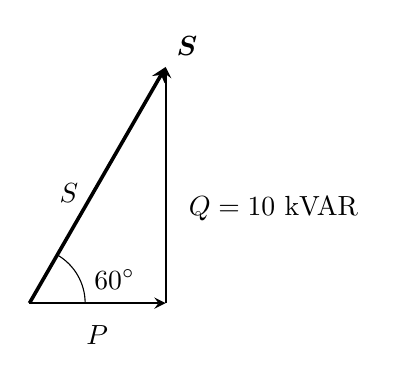
\begin{tikzpicture}
\draw[line width=1.3pt,-stealth] (0, 0) -- (1.73, 3) node[anchor = south west] {$\bm{S}$};
\draw (0.5, 1.4) node[]{$S$};
\draw[line width=0.8pt,-stealth] (0, 0) -- (1.73, 0);
\draw (0.86, -0.4) node[]{$P$};
\draw[line width=0.8pt,-stealth] (1.73, 0) -- (1.73, 3);
\draw (1.9, 1.2) node[anchor = west]{$Q=10 \ \textrm{kVAR}$};
\draw (0.707,0) arc (0:60:0.707);
\draw (0.7, 0.3) node[anchor = west]{$60^\circ$};
\end{tikzpicture}
\end{figure}
We can find average power using the equation
$$\tan(60^\circ) = \frac{10\ \textrm{kVAR}}{P}$$
Solving for $P$, we get $P = 5.77$ kW.

\section{Power Triangle}
Given $P = 4$ W and a power factor of 0.8 leading, draw the power triangle and find $S$ and $Q$.
\subsection*{Solution}
$\arccos(0.8) = 36.87^\circ$, but since current leads, $\alpha_i > \alpha_v \Rightarrow (\alpha_v - \alpha_i) < 0$, so the reactive power is negative:
\begin{figure}[H]
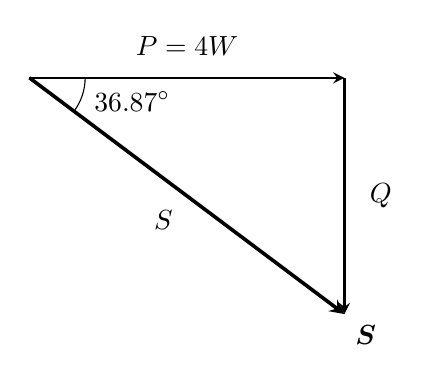
\begin{tikzpicture}
\draw[line width=1.3pt,-stealth] (0, 0) -- (4, -3) node[anchor = north west] {$\bm{S}$};
\draw (1.7, -1.8) node[]{$S$};
\draw[line width=0.8pt,-stealth] (0, 0) -- (4, 0);
\draw (2, 0.4) node[]{$P=4 W$};
\draw[line width=0.8pt,-stealth] (4, 0) -- (4, -3);
\draw (4.2, -1.5) node[anchor = west]{$Q$};
\draw (0.707,0) arc (0:-36.87:0.707);
\draw (0.7, -0.3) node[anchor = west]{$36.87^\circ$};
\end{tikzpicture}
\end{figure}
The apparent power can be found using the equation
$$\cos(36.87^\circ) = \frac{4\textrm{W}}{S} \Rightarrow S = 5 \ \textrm{VA}$$
The reactive power could be found using the pythagorean theorem: $Q = -3$ VAR.


\section*{Complex Power in RLC Circuit}
Find the average power, reactive power, apparent power, and power factor. \\ \\
\begin{circuitikz}[american, cute inductors] \draw
(0, 0) to[vsource, invert, l=$v(t) {=} 200\cos(2\pi60t) \textrm{V}$] (0, 3) to[R=$2\Omega$] (3, 3) to[C=$20\mu\textrm{F}$] (3, 0)
(3, 3) to[L=$3\textrm{mH}$] (6, 3) to[R=$5\Omega$] (6, 0) to[short] (0, 0)
;
\end{circuitikz} \\ \\
\subsection*{Solution}
The total impedance is
$$\bm{Z} = 2 + \frac{1}{j\cdot120\pi\cdot20\mu\textrm{F} + \frac{1}{j\cdot120\pi\cdot3\textrm{mH} + 5}} = 7.079 + 0.948j \ \Omega$$
The voltage is $\bm{V} = 200 \angle 0^\circ$ V, and the current is $\bm{I} = \frac{\bm{V}}{\bm{Z}} = 27.76 - 3.72j = 28 \angle -7.62^\circ \ \textrm{A}$.
The power factor is
$$PF = \cos(0^\circ - (-7.62^\circ)) = 0.9912, \  \textrm{lagging}$$
\\The apparent power is
$$S = \frac{200\cdot28}{2} = 2.8 \ \textrm{kVA}$$
The average power is
$$P = S\cdot PF = 2.8 \textrm{kVA}\cdot 0.9912 = 2.775 \ \textrm{kW}$$
The reactive power is
$$Q = S\cdot\sin(7.62^\circ) = 371 \ \textrm{VAR}$$


\newpage
\section*{References}
\begin{itemize}
\item M. Iordache. Class Lectures, Topic: ``Electric circuits.'' EEGR 2053, School of Engineering and Engineering Technology, LeTourneau University, 2025.
\item M. Iordache. 2024. EEGR 2053 Electric circuits [PowerPoint slides]. Available: \\ https://mviordache.name/EEGR2053/index.html
\item T. L. Floyd and D. M. Buchla, Principles of Electric Circuits: Conventional Current, 10th ed. Hoboken, NJ: Pearson Education, 2020.
\item O. Ortiz. 2025. ENGR 2053 Intro to electric circuits [PowerPoint slides].
\end{itemize}

\end{document}









